\documentclass{ieeeojies}
\usepackage{cite}
\usepackage{amsmath,amssymb,amsfonts}
\usepackage{algorithmic}
\usepackage{graphicx}
\usepackage{textcomp}
\usepackage{array}
\usepackage[table]{xcolor}
\usepackage{multirow}
\usepackage{multicol}
\usepackage{float}
\usepackage{amsmath}
\usepackage{mathabx}

\def\BibTeX{{\rm B\kern-.05em{\sc i\kern-.025em b}\kern-.08em
    T\kern-.1667em\lower.7ex\hbox{E}\kern-.125emX}}



\begin{document}
\title{MINERAL PRICE FORECASTING USING TIME SERIES ANALYSIS TECHNIQUES}

\author{\uppercase{Mai Quoc Bao}\authorrefmark{1},
\uppercase{Bui Huu Bang\authorrefmark{2}, Tran Minh Hoang\authorrefmark{3}, Vo Ngoc Le Xuan\authorrefmark{4},\\ Tran Kim Thanh}\authorrefmark{5}}

\address[1]{Faculty of Information Systems, University of Information Technology, (e-mail: 21521850@gm.uit.edu.vn)}
\address[2]{Faculty of Information Systems, University of Information Technology, (e-mail: 21520151@gm.uit.edu.vn)}
\address[3]{Faculty of Information Systems, University of Information Technology, (e-mail: 21522101@gm.uit.edu.vn)}
\address[4]{Faculty of Information Systems, University of Information Technology, (e-mail: 21521692@gm.uit.edu.vn)}
\address[5]{Faculty of Information Systems, University of Information Technology, (e-mail: 21522605@gm.uit.edu.vn)}

\markboth
{Author \headeretal: Mai Quoc Bao, Bui Huu Bang, Tran Minh Hoang, Vo Ngoc Le Xuan, Tran Kim Thanh}
{Author \headeretal: Mai Quoc Bao, Bui Huu Bang, Tran Minh Hoang, Vo Ngoc Le Xuan, Tran Kim Thanh}

\begin{abstract}
In recent decades, precious metals have been maintaining their appeal among investors, especially gold, platinum and silver. Along with that, metal price prediction problems and models are constantly being born and improved with higher and higher accuracy. However, depending on the world economic context and the advancement of data analysis techniques, predictive models will produce different results. To solve this problem, our team will build and evaluate price forecasting models in parallel with the following 10 algorithms: Linear Regression, ARIMA, RNN, GRU, LSTM, FFT, TBATS, SES, N-HiTS, PatchTST; Along with that are 3 model testing methods: MAPE, RMSE, MAE.
\end{abstract}

\begin{keywords}
Linear Regression – Linear Regression, ARIMA – Autoregressive Integrated Moving Average, RNN – Recurrent Neural Network, GRU – Gated Recurrent Unit, LSTM – Long Short Term Memory, FFT – Fast Fourier Transform, TBATS – (Trigonometric seasonality, Box-Cox transformation, ARMA errors, Trend, Seasonal components), SES – Simple Exponential Smoothing, N-HiTS – Neural Hierarchical Interpolation for Time Series, PatchTST – Patch Time Series Transformer, MAPE – Mean Absolute Percentage Error,  RMSE – Root Mean Squared Error, MAE – Mean Absolute Error.
\end{keywords}

\titlepgskip=-15pt

\maketitle

\section{Introduction}
\label{sec:introduction}
The volatility of gold(Au), silver(Ag) and platinum(Pt) prices has always been a hot spot in the investment and financial sectors. Predicting the price of these precious metals is not only important in supporting investors' investment decisions and market analysis, but also in providing detailed and accurate information on price movements, which greatly improves business performance and risk management in related areas such as securities securities and currencies.\\
Predicting the price of precious metals like gold not only focuses on predicting the global price of 1 day but also predicting prices in the future such as 3 to 5 months later, predicting price fluctuations, fluctuation trends, the relationship of prices of metals, ... Therefore, many professional forecasting websites have been established such as Bloomberg, Kitco, LBmMA,...\\
By comparing and testing many forecasting methods and models from classic to the latest, the research team expects to find the model and algorithm with the best results to flexibly meet the increasing demand of the market. Our research paper uses a dataset from the MetalPriceAPI website to derive historical recorded prices of gold, platinum, and silver (denominated in USD).


\section{Related Works}
The study, by authors Tawum Juvert Mbah, Haiwang Ye, Jianhua Zhang & Mei Long \cite{b1}, selected six factors influencing the limestone market to simulate and predict future price trends, including cement, gold, coal, energy, interest rates, and limestone prices. The study uses two advanced deep neural network models, RNN and ARIMA, to simulate and predict limestone prices. The results showed that the ARIMA model had better predictions than the RNN model about the trend and price movements of limestone. The main difference between these two models lies in the fact that the ARIMA model is capable of producing more accurate results and less training time than the RNN model. Therefore, the ARIMA network proved to be a sophisticated and effective method in modeling, analyzing, and predicting the price of the limestone market.\\
The study by Bojun Yin, Renguang Zuo, Yihui Xiong \cite{b2}, used a GRU model to create a Mineral Prospectivity Mapping (MPM), using data from Baguio County, Philippines. The results obtained underscore the effectiveness of the GRU model in MPM. The distinguished peak areas exhibit a close spatial relationship with known mineral deposits, providing important information for further mining activities in the study area.\\
There is also research by F.Javier Galán-Sales, Pablo Reina-Jiménez, Manuel Carranza-García, José María Luna-Romera \cite{b3}, which investigates the potential of using FFT as a characteristic transformational tool to improve the accuracy and efficiency of time series forecasting models. The team's results show that the use of FFT as a characterization transformation tool is superior to traditional characterization transformation methods in predicting computational accuracy and efficiency. 
\\
\section{Materials}
\subsection{Dataset}

The trio of datasets showing the prices of three precious metals: gold, silver and platinum for the period from January 1, 2018 to March 1, 2024 are sourced from APIs provided by https://metalpriceapi.com/.
After calling the API to get data, the team converted from json to csv and obtained 3 csv files including: Gold price, Silver price and Platinum price.\\
Within each dataset there are two columns:\\
• Date: date of data entry (YYYY-MM-DD) format.\\
• Value (USD per troy ounce): the price of the precious metal corresponds to the Date column (denomination USD).

\subsection{Descriptive Statistics}
\begin{table}[H]
  \centering
  \caption{Gold price, Silver price and Platinum price’s Descriptive Statistics}
\begin{tabular}{|>{\columncolor{red!20}}c|c|c|c|}
    \hline
     \rowcolor{red!20} & Gold price & Silver price & Platinum price \\ \hline
     Count & 2252 & 2251 & 2252 \\ \hline
     Mean & 1673.567 & 20.531 & 940.485\\ \hline
     Std & 262.337 & 4.131 & 106.855\\ \hline
     Min & 1178.57 & 12.112 & 591.46\\ \hline
     25\% & 1419.73 & 16.572 & 864.475\\ \hline
     50\% & 1768.317 & 21.584 & 930.843\\ \hline
     75\% & 1884.517 & 23.975 & 999.513\\ \hline
     Max & 2085.54 & 29.748 & 1306.684\\ \hline
\end{tabular}
\end{table}

\begin{figure}[H]
    \centering
    \begin{minipage}{0.23\textwidth}
    \centering
    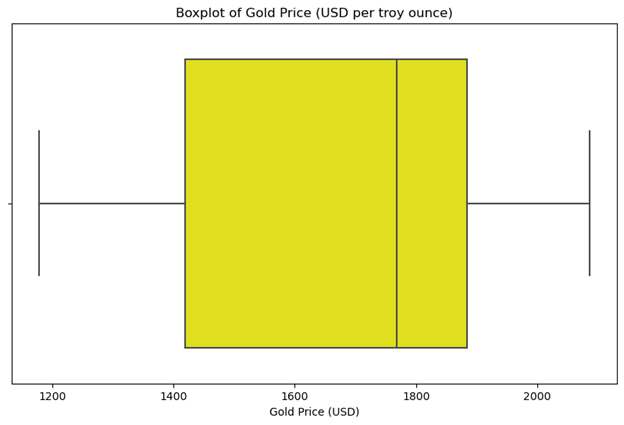
\includegraphics[width=1\textwidth]{bibliography/Figure/boxplot_gold.png}
    \caption{Gold price's boxplot}
    \label{fig:1}
    \end{minipage}
    \hfill
    \begin{minipage}{0.23\textwidth}
    \centering
    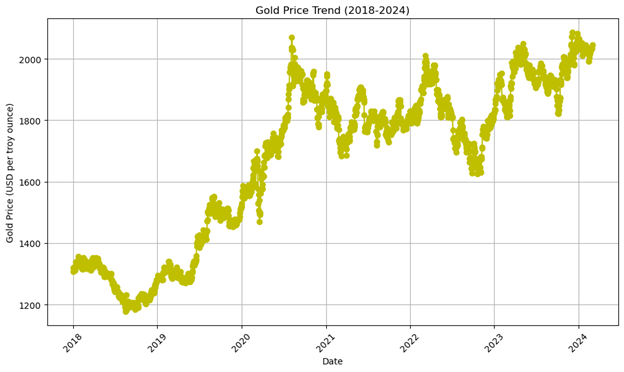
\includegraphics[width=1\textwidth]{bibliography/Figure/line_gold.png}
    \caption{Gold price's line chart}
    \label{fig:2}
    \end{minipage}
\end{figure}

\begin{figure}[H]
    \centering
    \begin{minipage}{0.23\textwidth}
    \centering
    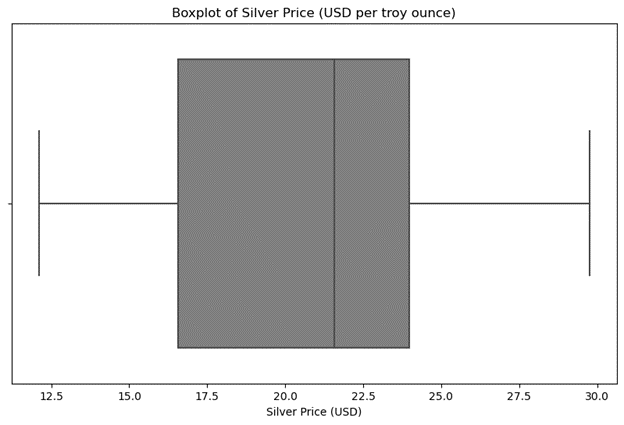
\includegraphics[width=1\textwidth]{bibliography/Figure/boxplot_silver.png}
    \caption{Silver price's boxplot}
    \label{fig:1}
    \end{minipage}
    \hfill
    \begin{minipage}{0.23\textwidth}
    \centering
    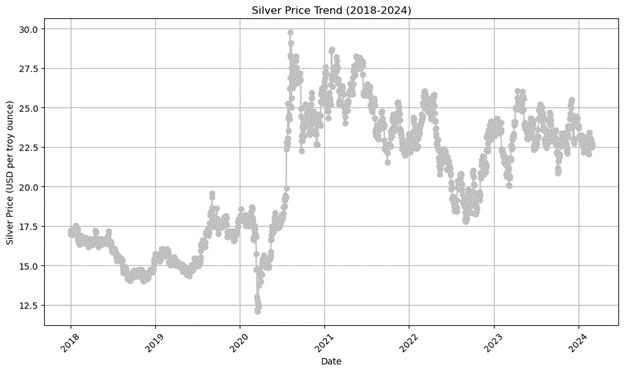
\includegraphics[width=1\textwidth]{bibliography/Figure/line_silver.png}
    \caption{Silver price's line chart}
    \label{fig:2}
    \end{minipage}
\end{figure}

\begin{figure}[H]
    \centering
    \begin{minipage}{0.23\textwidth}
    \centering
    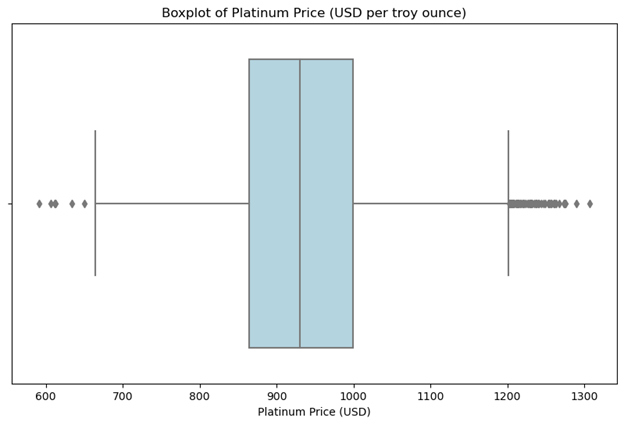
\includegraphics[width=1\textwidth]{bibliography/Figure/boxplot_pt.png}
    \caption{Platinum price's boxplot}
    \label{fig:1}
    \end{minipage}
    \hfill
    \begin{minipage}{0.23\textwidth}
    \centering
    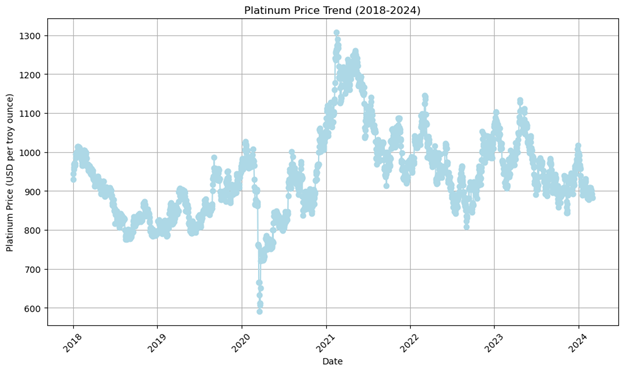
\includegraphics[width=1\textwidth]{bibliography/Figure/line_pt.png}
    \caption{Platinum price's line chart}
    \label{fig:2}
    \end{minipage}
\end{figure}
\subsection{Tools}
In the process of researching and analyzing data to forecast mineral prices, the team used several popular tools and software libraries, mainly implemented in the Python programming language. List of main tools and libraries used: Pandas, NumPy, Matplotlib, Seaborn, Scikit-learn,...

\section{Methodology}
\subsection{Linear Regression}
Linear regression, first introduced by statistician Sir Francis Galton in the late 19th century, is a statistical method used to model the relationship between a dependent variable and an independent variable (or more). Single linear regression has 1 independent variable, multiple linear regression has more than 1 independent variable.\\
It builds a linear model by finding a straight line (if it is univariate regression) or a hyperplane (if it is multivariate regression) that predicts the best based on a linear relationship so that the difference between the predicted and actual values is minimal. \\
Linear regression is widely applied to predict output values, considering the influence of variables in areas such as economics, finance, environment,...\\
Simple linear regression equation: 
\begin{samepage}
\[Y=\beta_0+\beta_1X_1+\varepsilon\]
\end{samepage}
Multiples linear regression equation with k independent variables:
\begin{samepage}
\[Y=\beta_0+\beta_1X_1+...+\beta_kX_k+\varepsilon\]
\end{samepage}
Where:\\
	\indent\textbullet\ Y is the dependent variable (Target Variable).\\
	\indent\textbullet\ \(X_1, X_2, \ldots, X_k\) are the independent (explanatory) variables.\\
	\indent\textbullet\ \(\beta_0\) is the intercept term.\\
	\indent\textbullet\ \(\beta_1,..., \beta_k\) are the regression coefficients for the independent variables.\\
	\indent\textbullet\ \(\varepsilon\) is the error term.

\subsection{ARIMA}
ARIMA, or self-regression integrated moving average model, is a method of statistical analysis that uses time series data to better understand a data set or predict future trends. In general, ARIMA is a combined model of 2 self-regression processes and a sliding average. Past data will be used to forecast future data.\\
The ARIMA model stands for Auto Regression (AR), Moving Average (MA) and Integrated Differential (I) integration. \\
\indent\textbullet\ \textbf{Integrated (I) d:} A process of co-integration, or falsehood, to compare the differences between d observations.
\\
\indent\textbullet\ \textbf{Auto regression (AR) p}: This is a self-regression component consisting of the set of lags of the current variable. The latency of degree p is the value that goes back to the past p time step of the string. The long or short delay in the AR process depends on the delay parameter p. 
\\
\indent\textbullet\ \textbf{Moving average (MA) q}: The process of moving average (MA) q is understood as the process of shifting or changing the average value of the series over time. The moving average process will find a linear connection between the current data and q of the previous t-error.
\\
The ARIMA regression equation(p, d, q) can be expressed as:
Simple linear regression equation: 
\begin{samepage}
\[\Delta x_t = \sum_{i=1}^{p} \alpha_i \Delta (x_{t-i}) +  \sum_{i=1}^{q} \beta_i \varepsilon_{t-i}\]
\end{samepage}

\subsection{RNN}
An RNN (Recurrent neural network) is a type of neural network commonly used for sequential data such as time series. RNNs use the output of the previous step as input to the current step, whereas traditional Neural Networks all inputs and outputs are independent of each other. 
\\
The main and most important characteristic of RNNs is the hidden state. This state remembers the previous input of the network. It uses the same weight for the input of each layer in the network.
\\
RNN computes the hidden state denoted as \( h_t \) based on the current input \( x_t \) and the previous hidden state \( h_{t-1} \):

\[
h_t = \sigma_h(W_{xh} x_t + W_{hh} h_{t-1} + b_h)
\]

The output \( y_t \) of the RNN is computed based on the current hidden state \( h_t \):

\[
y_t = \sigma_y(W_{hy} h_t + b_o)
\]
Where:\\

\begin{itemize}
  \item \( \sigma_h, \sigma_y \): Activation functions for the hidden layer and the output layer.
  \item \( W_{xh} \): Weight matrix from the input layer to the hidden layer.
  \item \( W_{hh} \): Weight matrix from the hidden layer to itself.
  \item \( W_{hy} \): Weight matrix from the hidden layer to the output layer.
\end{itemize}
These parameters are updated using Backpropagation. However, since RNNs operate on sequential data, they use Backpropagation Through Time (BPTT).

Unlike traditional backpropagation that only computes errors for the final output, BPTT calculates errors for each time step in the sequence and propagates them back through time, updating the parameters of the entire network to minimize the total error.


\subsection{GRU}
A gate-tode retrospective neural network (GRU) is a gate mechanism in regression neural networks, which is a simpler variant of Long Term Memory (LSTM) networks. The GRU can process sequential data such as text, articles, and time series.
\\
The GRU uses a gateway mechanism to selectively update the hidden state of the network at each time step. The gateway mechanism is used to control the incoming and outgoing data flow of the network. The GRU has 2 port mechanisms: the delete port and the update port. 
\\
The deletion portal decides how much of the previous state is retained, while the update portal decides how much of the same part of the old hidden state is the same as the old hidden state. The output of the GRU is computational based on the number of updated hidden states, making it possible for the model to 'remember' important information from the past and 'look' at new information to adjust to the current state.
The equation for calculating the delete port, update port, and hidden state number of the GRU is as follows: \\
 \textbf{Reset gate:} 

\[
R_t = \sigma(X_t W_{xr} + H_{t-1} W_{hr} + b_r)
\]
 \textbf{Update gate:} 
\[
Z_t = \sigma(X_t W_{xz} + H_{t-1} W_{hz} + b_z)
\]
Where:\\

\begin{itemize}
    \item $X_t$: input at the current time step.
    \item $H_{t-1}$: is the hidden state in the previous step.
    \item $W_{xr}, W_{xz} \in \mathbb{R}^{d \times h}$ and $W_{hr}, W_{hz} \in \mathbb{R}^{h \times h}$: weights.
    \item $b_r, b_z \in \mathbb{R}^{1 \times h}$: the cliché parameters.
    \item $\sigma$: sigmoid function so that the 2 obtained values belong to the interval $(0,1)$.
\end{itemize}

\vspace{-1em} % Adjust this value to reduce space
\begin{figure}[H]
    \centering
    \includegraphics[width=0.5\textwidth]{bibliography/Figure/GRU.jpg}
    \caption{GRU Model}
    \label{fig:GRU_Model}
\end{figure}


\subsection{LSTM}
Long short-term memory (LSTM) is a type of regression neural network (RNN) designed to solve the problem of disappearing gradients in traditional RNNs. The advantage of LSTM is its ability to handle long distances between information, making it useful in applications such as speech recognition, machine translation, and time series analysis.
\\
An LSTM unit consists of a cell, an input port, an output port, and a forgotten port. The cell remembers information for long periods of time, while the gates control the flow of information into and out of the cell. The gateway forgets to decide what information to ignore, the input gateway decides what new information to store, and the output port decides what information to output, helping the LSTM network maintain useful long-term dependencies to make predictions.
\\
The forgotten port deletes information that is no longer useful from the memory cell. The equation of the forgotten gate:\\
\begin{equation*}
    f_t = \sigma(W_f [h_{t-1}, x_t] + b_f)
\end{equation*}

Where:
\begin{itemize}
    \item $\sigma$: Sigmoid activation function
    \item $W_f$ and $b_f$: Weights and biases of the forget gate
\end{itemize}

The input gate will add useful information to the memory cell. The equation for the input gate is:
\\
\begin{align*}
    i_t &= \sigma(W_i [h_{t-1}, x_t] + b_i) \\
    \tilde{C}_t &= \tanh(W_c [h_{t-1}, x_t] + b_c) \\
    C_t &= f_t \cdot C_{t-1} + i_t \cdot \tilde{C}_t
\end{align*}

Where:
\begin{itemize}
    \item $i_t$: Input at time t
    \item $C_{t-1}$: Memory cell at time t-1
    \item $W_c, b_c$: Weights and biases of the memory cell
    \item $\tanh$: Tanh activation function
\end{itemize}

The output gate will extract useful information from the current memory cell to present as output. The equation for the output gate is:

\begin{equation*}
    o_t = \sigma(W_o [h_{t-1}, x_t] + b_o)
\end{equation*}
    

\subsection{FFT}

The fast Fourier transform (FFT) is an extremely efficient algorithm for converting a time domain discrete signal to a frequency domain based on the discrete Fourier transform (DFT). The DFT transform analyzes a sequence of numbers into components at different frequencies. This transformation helps identify the main frequency components of the time series, thereby forecasting future values based on these components.

Discrete Fourier transform - DFT of a given discrete signal 
\[
x(n) = [x_0, x_1, \ldots, x_{N-1}]
\] 
calculated by the following expression:

\[
X(k) = 
\begin{cases} 
\sum_{n=0}^{N-1} x(n) e^{-i \frac{2\pi}{N} kn} & \text{If } 0 \le k \le N-1 \\
0 & \text{If } k \text{ belongs to the rest}
\end{cases}
\]

Where: \( i \) is the imaginary unit.

DFT transform calculation has a complexity of \(O(N^2)\).

FFT was created to overcome the processing speed of DFT. 

Suppose that the sequence \(x(n)\) has length \( N = 2^i \), if there is no form of power 2, then add some form 0 after the sequence \(x(n)\). The basic principle on which FFT algorithms are based is to divide the sample DFT N into smaller DFTs continuously. 

For \( N = 2^i \), we will first divide the sample DFT of size \( N \) into \( N/2 \) sample DFTs, then divide each of these sample DFTs into \( N/4 \) samples, and so on until the size of the DFT is \( N = 2 \). In essence, it is recursive. Hence, the complexity of the FFT is defined as \( O(N \log_2(N)) \).

FFT algorithm: 
\[
X(k) = \sum_{n=0}^{\frac{N}{2}-1} x_{2n} e^{-i \frac{2\pi}{N} (2n) k} + \sum_{n=0}^{\frac{N}{2}-1} x_{2n+1} e^{-i \frac{2\pi}{N} (2n+1) k}
\]

\subsection{N-HiTS}
The N-HiTS (Neural Hierarchical Interpolation for Time Series) algorithm is an advanced method for time series forecasting, built on the Neural Basis Expansion Analysis (N-BEATS) framework. N-HiTS aims to improve accuracy and computational efficiency, particularly for long-term forecasts. It introduces key innovations such as multi-rate signal sampling and hierarchical multi-rate aggregation to build forecasts in a hierarchical manner, reducing computational requirements while enhancing accuracy.

\subsubsection{Multi-Rate Signal Sampling}

Each block in the N-HiTS architecture uses a MaxPool layer with kernel size \( k_\ell \) to focus on different scales of the input signal. This multi-rate sampling ensures that each block analyzes the components of the input at different sample rates, allowing blocks with larger kernels to focus on larger-scale components and blocks with smaller kernels to focus on finer details. Formally, with input \( y_{t-L:t,\ell} \) for block \( \ell \), the output after pooling is:
\[
y^{(p)}_{t-L:t,\ell} = \text{MaxPool}(y_{t-L:t,\ell}, k_\ell)
\]

\subsubsection{Nonlinear Regression}

After multi-rate sampling, each block performs nonlinear regression to compute forward \( \theta^f_\ell \) and backward \( \theta^b_\ell \) coefficients for interpolation. These coefficients are generated using a multilayer perceptron (MLP) that processes the pooled input:
\[
h_\ell = \text{MLP}_\ell(y^{(p)}_{t-L:t,\ell})
\]
\[
\theta^f_\ell = \text{Linear}^f(h_\ell)
\]
\[
\theta^b_\ell = \text{Linear}^b(h_\ell)
\]

\subsubsection{Hierarchical Interpolation}

In typical multi-horizon forecasting models, the output size directly corresponds to the forecast horizon \( H \). This often leads to high computational costs and increased model complexity. N-HiTS mitigates this by using hierarchical interpolation, where the magnitude of the forecast coefficients \( \theta^f_\ell \) is controlled by the expression rate \( r_\ell \) as follows:
\[
|\theta^f_\ell| = \lceil r_\ell H \rceil
\]

To recover the full forecast horizon \( H \), interpolation is applied:
\[
\hat{y}_{\tau,\ell} = g(\tau, \theta^f_\ell), \forall \tau \in \{t+1, ..., t+H\}
\]
\[
\tilde{y}_{\tau,\ell} = g(\tau, \theta^b_\ell), \forall \tau \in \{t-L, ..., t\}
\]

The interpolation function \( g \) can vary in smoothness, with options such as nearest neighbor, piecewise linear, and cubic interpolation explored.

\subsubsection{Block and Stack Structure}

N-HiTS is composed of multiple blocks organized into stacks, with each stack designed to specialize in capturing different characteristics of the time series data. Each block contains an MLP that produces backcast \( \tilde{y}_{t-L:t,\ell} \) and forecast \( \hat{y}_{t+1:t+H,\ell} \) outputs. The blocks are connected in a doubly residual stacking manner, allowing each block to refine the input signal for subsequent blocks and gradually improve the forecasts.
Formally, the input to block \( \ell \) in stack \( s \) can be represented as:
\[
y_{t-L:t,\ell} = y_{t-L:t} - \sum_{i=1}^{\ell-1} \tilde{y}_{t-L:t,i}
\]

The output of each block is then aggregated to form the final forecast:
\[
\hat{y}_{t+1:t+H} = \sum_{\ell=1}^{B} \hat{y}_{t+1:t+H,\ell}
\]
    
\subsection{TBATS}
TBATS is an advanced time series prediction model, improved upon the BATS model, and developed by Rob J. Hyndman and Nikolaos Kourentzes. The TBATS model was created in 2011 with the aim to forecast time series with multiple seasonal cycles (cycles in hours, days, quarters, years,..). TBATS can handle complex crop forms such as non-integer, non-nested, and long-cycle seasons.
 \\
 TBATS is less common and less commonly used than other models in the ARIMA model genealogy. TBATS consists of 5 components:\\
\indent\textbullet\ \textbf{Trigonometric seasonality: } uses trigonometric transformation (sin-cos) to model seasonal factors with a fixed frequency.
\\
\indent\textbullet\ \textbf{Box-Cox transformation:}: handles the heterogeneity of data, which improves data distribution and makes their variance more uniform. 
\\
\indent\textbullet\ \textbf{ARMA errors (slippage average combined self-regression error):}: helps predict random errors that are not seasonal.\\
\indent\textbullet\ \textbf{Trend components:} shows a model that predicts an upward and downward trend.\\
\indent\textbullet\ \textbf{Seasonal components: } remove cyclic fluctuations from data.
\\
Formula:\\
\begin{itemize}
    \item \textbf{Box-Cox transformation:}
    \begin{itemize}
        \item Linear case:
        \[
        y_t^{(\omega)} =
        \begin{cases}
        \frac{y_t^\omega - 1}{\omega}, & \omega \neq 0 \\
        \log y_t, & \omega = 0
        \end{cases}
        \]
        \[
    y_t^{(\omega)} = l_{t-1} + \phi b_{t-1} + \sum_{i=1}^{T} s_{t-m_i}^{(i)} + d_t
    \]
        
        \item Non-linear case:
        \[
        y_t^{(\omega)} = w' x_{t-1} + \varepsilon_t
        \]
        \[
        x_t = F x_{t-1} + g \varepsilon_t
        \]

        Where \( m_1, \ldots, m_T \) refers to seasonal cycles, \( l_t \) is the local level of the cycle \( t \), \( st^(i) \) represents the seasonal composition at time \( t \), \( \mathbf{w'} \) is a vector current, \( \mathbf{g} \) is a column vector, \( \mathbf{F} \) is a matrix, and \( \mathbf{x}_t \) is the unobserved state vector at time \( t \) (future). 
    \end{itemize}
    \item \textbf{The function handles with smoothing method – trend damping, finding ARMA coefficients, specific level:}
    \begin{align*}
    l_t &= l_{t-1} + \phi b_{t-1} + \alpha d_t \\
    d_t &= \sum_{i=1}^{p} \varphi_i d_{t-i} + \sum_{i=1}^{q} \theta_i \varepsilon_{t-i} + \varepsilon_t \\
    b_t &= (1 - \phi)b + \phi b_{t-1} + \beta d_t
    \end{align*}
    Where \( b_t \) is the short-term trend in the period \( t \), \( d_t \) is about the coefficient ARMA(\( p \), \( q \)) and the error \( \varepsilon_t \) is taken from the white noise process with mean = 0 and fixed variances \( \sigma^2 \), \( \alpha \) and \( \beta \) and \( \gamma_i \) (\( i = 1, \ldots, T \)) are the smoothing coefficients, \( i \) is the \( i \)-component coefficient of the sliding average (MA). The Gardener & McKenzie smoothing trend with \( \phi \) parameter is used in the Snyder direction to make \( b_t \).

    
    \item \textbf{Trigonometric transform function:}
    \[
    s_t^{(i)} = \sum_{j=i}^{k_i} s_{j,t}^{(i)}
    \]
    \[
    k_i = 
    \begin{cases} 
    \frac{m_i}{2} & \text{if the value of season i is even,} \\
    \frac{(m_i - 1)}{2} & \text{if the value of season i is odd}
    \end{cases}
    \]
    \begin{align*}
    s_{j,t}^{(i)} &= s_{j,t-1}^{(i)} \cos \lambda_j^{(i)} + s_{j,t-1}^{*(i)} \sin \lambda_j^{(i)} + \gamma_1^{(i)} d_t \\
    s_{j,t}^{*(i)} &= -s_{j,t-1} \sin \lambda_j^{(i)} + s_{j,t-1}^{*(i)} \cos \lambda_j^{(i)} + \gamma_2^{(i)} d_t \\
    \lambda_j^{(i)} &= 2\pi j / m_i
    \end{align*}
In particular, \( \gamma_1 \) and \( \gamma_2 \) are the smoothing parameters, \( s_{j,t}^{(i)} \) are the random growth rates in the interval \( s_j^{*(i)} \).


\end{itemize}





\begin{figure}[H]
    \centering
    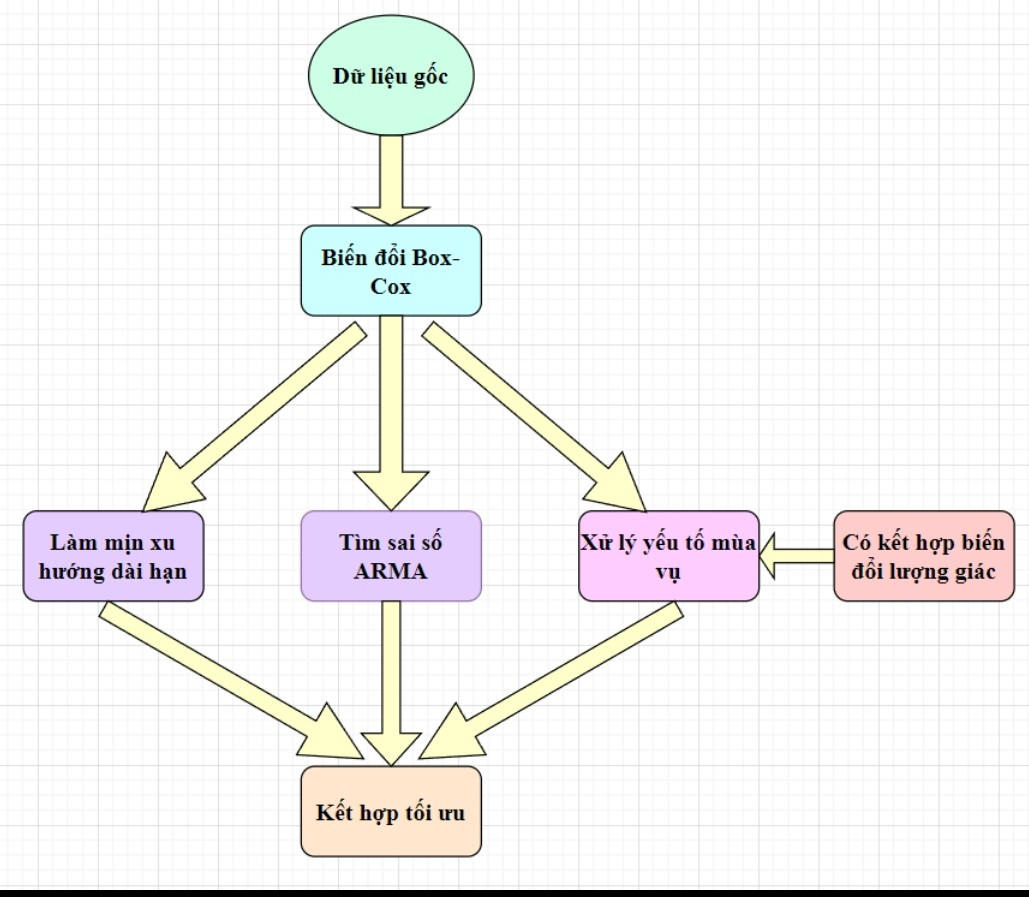
\includegraphics[width=0.5\textwidth]{bibliography/Figure/tbats.png}
    \caption{TBATS Work-Flow}
    \label{fig:tbats_workflow}
\end{figure}

\subsection{SES}
Simplified Exponential Smoothing (SES) is a simple and effective time forecasting method used to smooth time series data and predict future values. SES is especially useful when short-term forecasting is needed in data that does not have a clear trend or seasonality. This method works by applying an exponentially decreasing weight to previous observations, which smooths out random fluctuations in the data. 
\\
Formula: 
\begin{equation}
s_t = \alpha x_t + (1 - \alpha) s_{t-1} + \alpha (x_t - s_{t-1})
\end{equation}

\begin{itemize}
  \item $s_t$: predict value
  \item $s_{t-1}$: previous predict value
  \item $\alpha$: smoothing coefficient $(0 < \alpha < 1)$
  \item $t$: timestamp
\end{itemize}
When the value of \( \alpha \) is large (close to 1), the degree of smoothing decreases. This means that the SES algorithm will have less smoothing and will react more strongly to the most recent changes in the data. The predicted values will be close to the most recently observed values.

\subsection{N-HiTS}
N-HiTS, an enhanced method of N-BEATS for more accurate and efficient prediction for long-distance forecasting. N-HiTS uses multi-speed sampling and multi-scale composite combinations to build hierarchical forecasts, reducing computational requirements. Similar to N-BEATS, it uses a local non-linear projection onto base functions through blocks organized into stacks. 
\\
Each block of the perceptron multilayer generates coefficients for predicted and reverse predicted outputs. The method consists of S stacks, each with B cubes containing MLP to predict forward and backward base function coefficients. \\
N-HiTS combines the following ideas and techniques:
\begin{enumerate}
  \item \textbf{Hierarchical Forecasting:} This method performs hierarchical forecasting, meaning that the forecast is carried out through different levels of the forecast length. This helps reduce computational requirements and improve the accuracy of the forecast.
  
  \[
  y_t = g(\theta_f)
  \]
  
  \( y_{t+1:t+H} \) is a series of forecast values in the future from time \( t+1 \) to \( t+H \).

  \( \theta_f \) are the parameters of the model, including the coefficients of the base and backcast models.

  \( g \) is the time series model function that forecasts future values.

  \item \textbf{N-HiTS Sampling:} N-HiTS uses multi-scale temporal sampling to create a comprehensive representation of the data, improving the efficiency and accuracy of the model.

  \item \textbf{Nonlinear Base Projection:} In N-HiTS, nonlinear base projection is performed to improve the model. Each block consists of a multilayer perceptron (MLP) to create the base forecast and backcast through a shared projection.

  \item \textbf{Temporal Interpolation:} To forecast data in both the short and long term, N-HiTS interpolates the time series data. Because the forecast is carried out in multiple steps, it provides a better temporal interpolation function that combines the backcast and forecast across the required time horizon.
\end{enumerate}


\subsection{PatchTST}
PatchTST is a model that uses Transformers for multivariate forecasting and self-supervised representation learning. It is based on two main components:
\begin{enumerate}
    \item \textbf{Patching:} Segmentation of time series into small subseries-level segments, used as input tokens for the Transformer.
    \item \textbf{Channel-independence:} Each channel contains a single univariate time series, sharing the same embedding and Transformer weights across all series.
\end{enumerate}

The PatchTST architecture uses the vanilla Transformer encoder, where each univariate series of length \( L \) is segmented into patches, fed independently into the Transformer, and produces \( T \) future values \( (x_{L+1}, \ldots, x_{L+T}) \).

\ 
\\
\begin{figure}[H]
    \centering
    \includegraphics[width=0.5\textwidth]{bibliography/Figure/PatchTST.png}
    \caption{PatchTST Model}
    \label{fig:PatchTST_Model}
\end{figure}
The multivariate time series data \( x \in \mathbb{R}^{M \times L} \) is segmented into univariate series \( x^{(i)} \in \mathbb{R}^{1 \times L} \) for \( i = 1, \ldots, M \), and then fed into the Transformer Backbone for processing. The forward process is independent, and the output predictions \( \hat{x}^{(i)} \in \mathbb{R}^{1 \times T}, i = 1, \ldots, M \) are concatenated to produce the final output \( \hat{x} \in \mathbb{R}^{M \times T} \).

PatchTST has two variants:
\begin{itemize}
    \item \textbf{Supervised PatchTST:} Uses labeled data.
    \item \textbf{Self-Supervised PatchTST:} Does not require labeled data.
\end{itemize}
\section{Result}
\subsection{Evaluation Metrics}
\begin{enumerate}
    \item \textbf{Mean Absolute Percentage Error} (MAPE) is the average of the absolute percentage differences between the actual and predicted values.
    \begin{align*}
    MAPE &= \frac{1}{n} \sum_{i=1}^n \left|\frac{y_i - \hat{y}i}{y_i}\right| \cdot 100 \
    \end{align*}
    \item \textbf{Root Mean Square Error} (RMSE) is the square root of the mean of the squared differences between the actual and predicted values.
    \begin{align*}
    RMSE &= \sqrt{\frac{1}{n} \sum_{i=1}^n (y_i - \hat{y}i)^2} \
    \end{align*}
    \item \textbf{Mean Average Error} (MAE) is the average of the absolute differences between the actual and predicted values.
    \begin{align*}
    MAE &= \frac{1}{n} \sum_{i=1}^n |y_i - \hat{y}i| \
    \end{align*}
\end{enumerate}

\indent Where:
\begin{itemize}
    \item $n$ is the total number of observations
    \item $y_i$ is the $i$-th actual observation
    \item $\hat{y}_i$ is the $i$-th predicted observation
\end{itemize}

\subsection{Experimental Results and Evaluation}

\section{Conclusion}

\indent Horizontally, considering the gold price data, the best ratio for the models is … with the highest number of best results being …, the second best ratio is … (… times), and the worst ratio is … (… times). Similarly, for the platinum price data, the best ratio is … (… times), followed by the ratios … (… times) and … (… times). For the silver price data, the worst ratio is … (… times), followed by … (… times), and the best ratio is … (… times).

\indent Vertically, for each ratio, corresponding to each validation method, the we will select the top 3 forecasting models; top 1, 2, and 3 will be assigned scores of 3, 2, and 1, respectively. The model with the highest total score will be chosen. From there, the top 3 models for each data set will be selected.

\begin{table}[h!]
    \centering
    \resizebox{0.48\textwidth}{!}{
    \renewcommand{\arraystretch}{1.5}
    \small
    \begin{tabular}{|c|c|c|c|c|c|}
        \hline
        \textbf{Dataset} & \textbf{Ranking} & \textbf{Ratio 7:3} & \textbf{Ratio 8:2} & \textbf{Ratio 9:1} & \textbf{3 best models} \\ \hline
        \multirow{3}{*}{Gold price} & Top 1 & a & a & a & a \\ \cline{2-6} 
                                  & Top 2 &   &   &   &   \\ \cline{2-6} 
                                  & Top 3 &   &   &   &   \\ \hline
        \multirow{3}{*}{Platium price} & Top 1 & a & a & a & a \\ \cline{2-6} 
                                      & Top 2 &   &   &   &   \\ \cline{2-6} 
                                      & Top 3 &   &   &   &   \\ \hline
        \multirow{3}{*}{Silver price} & Top 1 & a & a & a & a \\ \cline{2-6} 
                                 & Top 2 &   &   &   &   \\ \cline{2-6} 
                                 & Top 3 &   &   &   &   \\ \hline
    \end{tabular}}
    \caption{\centering Vertically evaluating models ranking table}
    \label{table:models}
\end{table}

\indent Finally, after evaluating the models vertically across all three datasets, the group found that the best performing model is... Among the models that were expected to perform well, only the model... was selected as the best, while the models... and... did not have very good predictive results. Thus, the... model, according to the results, shows excellent learning capability with the potential to forecast the prices of the three precious metals in the future. Based on these findings, future research groups and data analysts can consider the models that can predict well and expand the research to forecast other metals or related fields, as well as improve the models to better serve academic and business needs.


\section*{Acknowledgment}
\addcontentsline{toc}{section}{Acknowledgment}
First and foremost, we would like to express our sincere gratitude to \textbf{Assoc. Prof. Dr. Nguyen Dinh Thuan} and \textbf{Mr. Nguyen Minh Nhut} for their exceptional guidance, expertise, and invaluable feedback throughout the research process. Their mentorship and unwavering support have been instrumental in shaping the direction and quality of this study. Their profound knowledge, critical insights, and attention to detail have significantly contributed to the success of this research.
\\This research would not have been possible without the support and contributions of our mentors. We would like to extend our heartfelt thanks to everyone involved for their invaluable assistance, encouragement, and belief in our research. Thank you all for your invaluable assistance and encouragement.

%% UNCOMMENT these lines below (and remove the 2 commands above) if you want to embed the bibliografy.
\begin{thebibliography}{00}
\bibitem{b1} Tawum Juvert Mbah, Haiwang Ye, Jianhua Zhang & Mei Long,
Using LSTM and ARIMA to Simulate and Predict Limestone Price Variations (06/01/2021).
\bibitem{b2} Bojun Yin, Renguang Zuo, Yihui Xiong, Mineral Prospectivity Mapping via Gated Recurrent Unit Model (25/11/2021).
\bibitem{b3} F.Javier Galán-Sales, Pablo Reina-Jiménez, Manuel Carranza-García, José María Luna-Romera, An Approach to Enhance Time Series Forecasting by Fast Fourier Transform (31/08/2023).

\end{thebibliography}
%%%%%%%%%%%%%%%


\EOD

\end{document}
